\documentclass[12pt]{beamer}
\usetheme{Boadilla}
\setbeamertemplate{footline}
{
  \leavevmode%
  \hbox{%
  \begin{beamercolorbox}[wd=.15\paperwidth,ht=2.25ex,dp=1ex,center]{author in head/foot}%
    \usebeamerfont{author in head/foot}\insertshortauthor
  \end{beamercolorbox}%
  \begin{beamercolorbox}[wd=.7\paperwidth,ht=2.25ex,dp=1ex,center]{title in head/foot}%
    \usebeamerfont{title in head/foot}\insertshorttitle
  \end{beamercolorbox}}%
  \begin{beamercolorbox}[wd=.15\paperwidth,ht=2.25ex,dp=1ex,center]{frame in head/foot}%
    \usebeamerfont{frame in head/foot} \insertframenumber{} / \inserttotalframenumber\hspace*{1ex}
  \end{beamercolorbox}}%
  \vskip0pt%


\newcommand\dbyd[2]{\frac{\mathrm d{#1}}{\mathrm d{#2}}}
\newcommand\dsided[2]{{\mathrm d{#1}}/{\mathrm d{#2}}}
\newcommand{\R}{\mathcal{R}}
\newcommand{\pmV}{p_{V}}
\newcommand{\pmI}{p_{I}}
\title{Intentional infection as a method of population level disease control}
\subtitle{Newborn infection}
\author{Roger Zhang}
\date{June 18th 2018}
\institute{McMaster University Department of Mathematics and Statistics}
\usepackage{paralist}
\begin{document}
\begin{frame}
\titlepage
\end{frame}
\begin{frame}
\frametitle{Motivation}
\begin{itemize}
\setlength\itemsep{10pt}
\item What are the historical examples?
\pause
\begin{itemize}
\setlength\itemsep{10pt}
\item Variolation of smallpox
\item Pox party
\end{itemize}
\pause
\item This method is out of date, banned in some places, why do we care?
\pause
\begin{itemize}
\setlength\itemsep{10pt}
\item In history, the mechanisms and benefits of intentional infection  on a population level was not quite understood.
\item New application to immunology, e.g. Transmissible vaccine.
\end{itemize}
\end{itemize}
\end{frame}
%%%%%%%%%%%%%%%%%%%%%%%%%%%%%%%%%%%%%%%%%%%%%%%%%%%%%%%%%%%%%%%
\begin{frame}
\frametitle{Method}
Standard SIR model:
\pause
\begin{equation}\label{1}
\begin{split}
\dbyd{S}{t}&=\mu- \beta SI-\mu S \,,\\
\dbyd{I}{t}&=\beta SI-\gamma I -\mu I\,,\\
\dbyd{R}{t}&=\gamma I-\mu R\,.
\end{split}
\end{equation}

Where $S$, $I$ and $R$ represent susceptible, infected and recovered.
\begin{itemize}
\setlength\itemsep{10pt}
\item $\mu$ is birth/death rate
\item $\beta$ is transmission rate
\item $\gamma$ is recovery rate
\end{itemize}
\end{frame}
%%%%%%%%%%%%%%%%%%%%%%%%%%%%%%%%%%%%%%%%%%%%%%%%%%%%%%%%%%%%%%%%%%%%%
\begin{frame}
\frametitle{Method}
Assumptions:
\begin{itemize}\itemsep10pt
\item No difference between intentionally infected and naturally infected individuals.
\item No disease induced mortality.
\item Birth and natural death rate are the same, the total population remains constant.
\item Latent period is short enough to be ignored.
\item All susceptible individuals are equally likely to be infected, and all infected individuals are equally infectious.
\end{itemize}
\end{frame}
%%%%%%%%%%%%%%%%%%%%%%%%%%%%%%%%%%%%%%%%%%%%%%%%%%%%%%%%%%%%%%%%%%
\begin{frame}
\frametitle{Method}
With intentional infection on newborn, 
\begin{equation}\label{2}
\begin{split}
\dbyd{S}{t}&=\mu(1-p)- \beta SI-\mu S \,,\\
\dbyd{I}{t}&=\beta SI+\mu p-\gamma I -\mu I\,,\\
\dbyd{R}{t}&=\gamma I-\mu R\,.
\end{split}
\end{equation}

Where $p$ is the proportion of newborn intentionally infected.
\end{frame}
%%%%%%%%%%%%%%%%%%%%%%%%%%%%%%%%%%%%%%%%%%%%%%%%%%%%%%%%%%%%%%%%%%%%%%
\begin{frame}
Non-dimensionalize the above system by scaling time, by
\begin{equation}
\tau=(\gamma+\mu)t \,,
\end{equation}

which yields

\begin{subequations}\label{3}
\begin{align}
\dbyd{S}{\tau}&=\epsilon(1-p)- \R_0  SI-\epsilon S \,,\\
\dbyd{I}{\tau}&=\R_0 SI+\epsilon p-I \,,
\end{align}
\end{subequations}

where $\epsilon=\frac{\mu}{\gamma+\mu}$, $\R_0=\frac{\beta}{\gamma+\mu}$.
\end{frame}
%%%%%%%%%%%%%%%%%%%%%%%%%%%%%%%%%%%%%%%%%%%%%%%%%%%%%%%%%%%%%%%%%%%%%%
\begin{frame}
\frametitle{Equilibria}
Solving equations above to find equilibria, we obtained only one set of solution,
\begin{subequations}
\begin{align}
\hat{S} &=\frac{1}{\R_0}-\frac{2p}{(\R_0 -1)+ \sqrt{(\R_0-1)^2+4\R_0 p}}\,, \label{Shat1}\\
\hat{I} &= \frac{\epsilon(\R_0 -1)+ \epsilon \sqrt{(\R_0-1)^2+4\R_0
    p}}{2\R_0}\,.\label{Ihat1}
\end{align}
\end{subequations}
\begin{itemize}
\item $\hat{I}\neq 0$ for all $p$ between 0 and 1. \item The equilibrium is an Endemic Equilibrium (EE).
\end{itemize}
\end{frame}
%%%%%%%%%%%%%%%%%%%%%%%%%%%%%%%%%%%%%%%%%%%%%%%%%%%%%%%%%%%%%%%%%%%%%%
\begin{frame}
\frametitle{Stability of Equilibria}

Jacobian Matrix,
\pause
\begin{equation}
\mathcal{J} =
\begin{bmatrix}
    \ -\R_0 I-\epsilon       & -\R_0 S \\
    \ \R_0 I       & \R_0 S-1 \\
\end{bmatrix} \,.
\end{equation}
\end{frame}
%%%%%%%%%%%%%%%%%%%%%%%%%%%%%%%%%%%%%%%%%%%%%%%%%%%%%%%%%%%%%%%
%%%%%%%%%%%%%%%%%%%%%%%%%%%%%%%%%%%%%%%%%%%%%%%%%%%%%%%%%%%%%%%%%%
\begin{frame}
\frametitle{What else do we need?}
\pause
\begin{itemize}\itemsep10pt
\item It is challenging to compare the results of this model to others for the purpose of observing any advantages.
\pause
\item Define `` Have advantage'' by comparing total number of deaths.
\pause
\item If intentionally infected cases have the same case fatality proportion (CFP) as naturally infected cases, then it will result in more deaths.
\begin{itemize}
\item We need to have separate CFP for each of them.
\end{itemize}
\pause
\item We need to divide $I$ into two separate infective classes. $V$ for intentionally infected class, $I$ for naturally infected class.
\end{itemize}
\end{frame}
%%%%%%%%%%%%%%%%%%%%%%%%%%%%%%%%%%%%%%%%%%%%%%%%%%%%%%%%%%%%%%%%%%
\begin{frame}
\frametitle{Model with disease induced mortality rate}

Therefore, our model becomes,
\begin{subequations}\label{eq:base_ODE}
\begin{align}
\dbyd{S}{\tau}&=\epsilon(1-p)- \R_0 S(V+I)-\epsilon S\,, \label{eq:S_by_tau}\\
\dbyd{V}{\tau}&=\R_0 SV+\epsilon p-V\,, \label{eq:V_by_tau}\\
\dbyd{I}{\tau}&=\R_0 SI-I\,, \label{eq:I_by_tau}\\
\dbyd{M}{\tau}&=\pmV(1-\epsilon) V+\pmI(1-\epsilon) I\,,\\
\dbyd{R}{\tau}&=(1-\pmV)(1-\epsilon) V+(1-\pmI)(1-\epsilon) I-\epsilon R\,,
\end{align}
\end{subequations}

Where $\pmV$ and $\pmI$ represent the CFP for intentionally infected and naturally infected cases, respectively.
\end{frame}
%%%%%%%%%%%%%%%%%%%%%%%%%%%%%%%%%%%%%%%%%%%%%%%%%%%%%%%%%%%%%%%%%%
\begin{frame}
\frametitle{Equilibria}

If $p\neq 0$, the only equilibrium is,
\begin{subequations}
\begin{align}
\hat{S}&= \frac{1}{\R_0}-\frac{2p}{(\R_0 -1)+ \sqrt{(\R_0-1)^2+4\R_0
         p}}\,, \label{eq:Shat}\\
\hat{V}&= \frac{\epsilon(\R_0 -1)+ \epsilon \sqrt{(\R_0-1)^2+4\R_0 p}}{2\R_0}\,, \label{eq:Vhat}\\
\hat{I}&=0\,. \label{eq:Ihat}
\end{align}
\end{subequations}

\begin{itemize}
\item Naturally infected cases cease to exist at EE.
\begin{itemize}
\item Helpful for disease eradication.
\end{itemize}
\end{itemize}
\end{frame}
%%%%%%%%%%%%%%%%%%%%%%%%%%%%%%%%%%%%%%%%%%%%%%%%%%%%%%%%%%%%%%%%%%%
%\begin{frame}
%By using the same method as the previous model, we %again showed that the equilibrium is stable. 
%\end{frame}
%%%%%%%%%%%%%%%%%%%%%%%%%%%%%%%%%%%%%%%%%%%%%%%%%%%%%%%%%%%%%%%%%%%%%%
\begin{frame}
\frametitle{Effect of intentional infection on total mortality}
\begin{center}
Smallpox
\end{center}
\begin{table}[H]\label{tab:params}
\begin{center}
\caption{Model parameters and smallpox values.}
\smallskip
\begin{tabular}{c|c|r}
{\bfseries Symbol} & {\bfseries Meaning} & {\bfseries Value} \\\hline
$\frac{1}{\mu}$ & Average lifespan & 50 years \\
$\frac{1}{\gamma}$ & Mean infectious period & 22 days \\
$\R_0$ & Basic reproduction number & 4.5\\
$\pmV$ & Intentionally infected CFP & 0.01\\
$\pmI$ & Naturally infected CFP & 0.3
\end{tabular}
\end{center}
\end{table}
\end{frame}
%%%%%%%%%%%%%%%%%%%%%%%%%%%%%%%%%%%%%%%%%%%%%%%%%%%%%%%%%%%%%%%%%%%%%
\begin{frame}
\frametitle{Effect of intentional infection on total mortality}
\framesubtitle{Mortality rate at EE}
\begin{equation}
\left. \dbyd{M}{\tau}\right|_{\rm EE}=\frac{\pmV(1-\epsilon)\epsilon(\R_0 -1)+ \pmV(1-\epsilon)\epsilon \sqrt{(\R_0-1)^2+4\R_0 p}}{2\R_0}\,,
\end{equation}
\pause
\begin{itemize}
\item Mortality rate at EE increases as $p$ increases.
\pause
\item In the long run, a larger proportion of intentional infection will lead to more deaths.
\end{itemize}
\end{frame}
%%%%%%%%%%%%%%%%%%%%%%%%%%%%%%%%%%%%%%%%%%%%%%%%%%%%%%%%%%%%%%%%%%%
%\begin{frame}
%\begin{figure}[H]
%  \centering
%  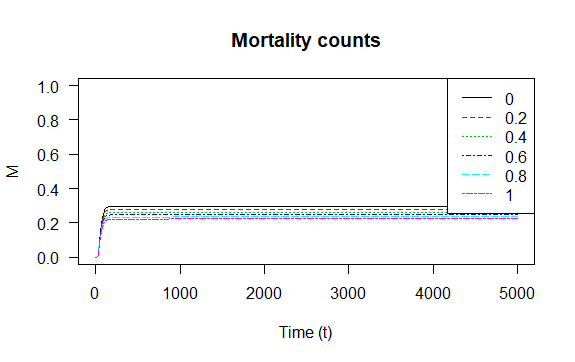
\includegraphics[width=0.6\textwidth]{Figures/Mortality_counts.png}
%  \caption{$\dbyd{M}{\tau}$ at EE as a function of $p$.}
%\label{fig:dMdt}
%\end{figure}

%Since the magnitude of $\dbyd{M}{\tau}$ is too small to be observed, we can hardly the the difference between the lines.
%\begin{itemize}
%\item $\pmV$ is too small
%\end{itemize}
%\end{frame}
%%%%%%%%%%%%%%%%%%%%%%%%%%%%%%%%%%%%%%%%%%%%%%%%%%%%%
%\begin{frame}
%To see the dynamics better, assume $\pmV=0.2$.
%\begin{figure}[H]
%  \centering
%  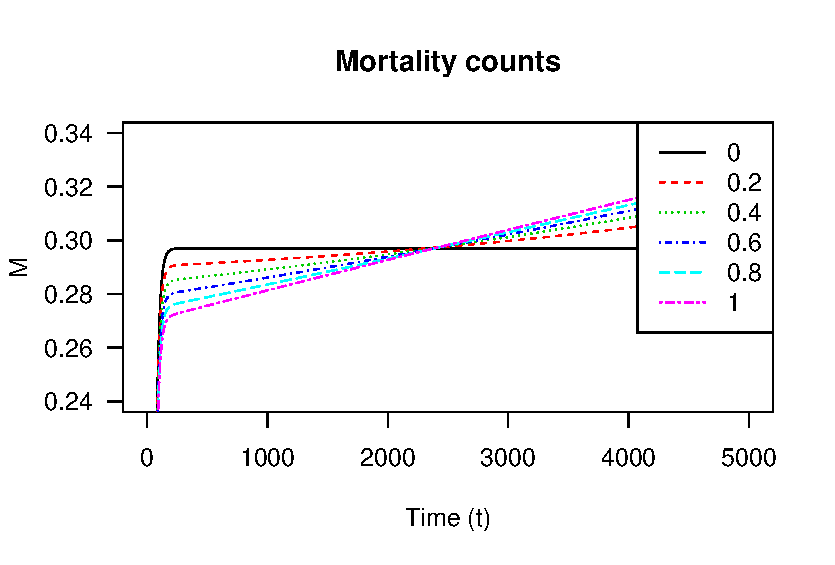
\includegraphics[width=0.9\textwidth]{Figures/Rplot.pdf}
%  \caption{$\dbyd{M}{\tau}$ at EE as a function of $p$.}
%\label{fig:dMdt}
%\end{figure}
%\end{frame}
%%%%%%%%%%%%%%%%%%%%%%%%%%%%%%%%%%%%%%%%%%%%%%%%%%%%%
\begin{frame}
\frametitle{Initial state being at equilibrium}

In history, intentional infection was introduced when the population is at equilibrium, which is the equilibrium for $p=0$.
\pause
\begin{subequations}
\begin{align}
\hat{S} &= \frac{1}{\R_0} \,,\\
\hat{V} &= 0\,,\\
\hat{I} &= \epsilon(1-\frac{1}{\R_0})
\end{align}
\end{subequations}
\end{frame}
%%%%%%%%%%%%%%%%%%%%%%%%%%%%%%%%%%%%%%%%%%%%%%%%%%%
\begin{frame}
\frametitle{Initial state being at equilibrium}
\begin{itemize}
\item What is the time it takes to reach the new EE?
\begin{itemize}
\item Need to define a threshold.
\end{itemize}
\end{itemize}
\pause

Since the new equilibrium has $\hat{I}=0$, define reaching equilibrium by $I\leq 10^{-6}$.
\end{frame}
%%%%%%%%%%%%%%%%%%%%%%%%%%%%%%%%%%%%%%%%%%%%%%%%%%%%%%
\begin{frame}
\begin{figure}[h]
  \centering
  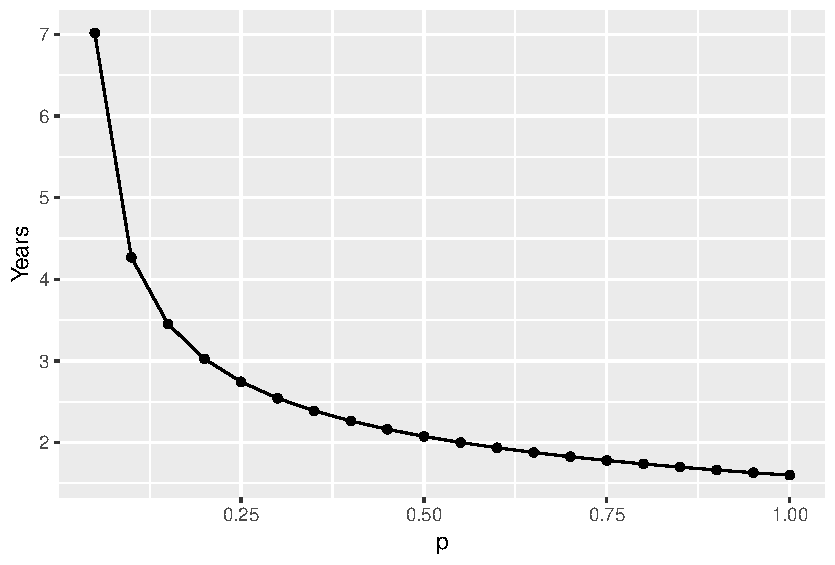
\includegraphics[width=0.9\textwidth]{Figures/Time_to_EE_plot.pdf}
  \caption{Determination of time taken to reach equilibrium}
\end{figure}
\end{frame}
%%%%%%%%%%%%%%%%%%%%%%%%%%%%%%%%%%%%%%%%%%%%%%%%%%%%%5
%\begin{frame}
%\begin{figure}[H]
%  \centering
%  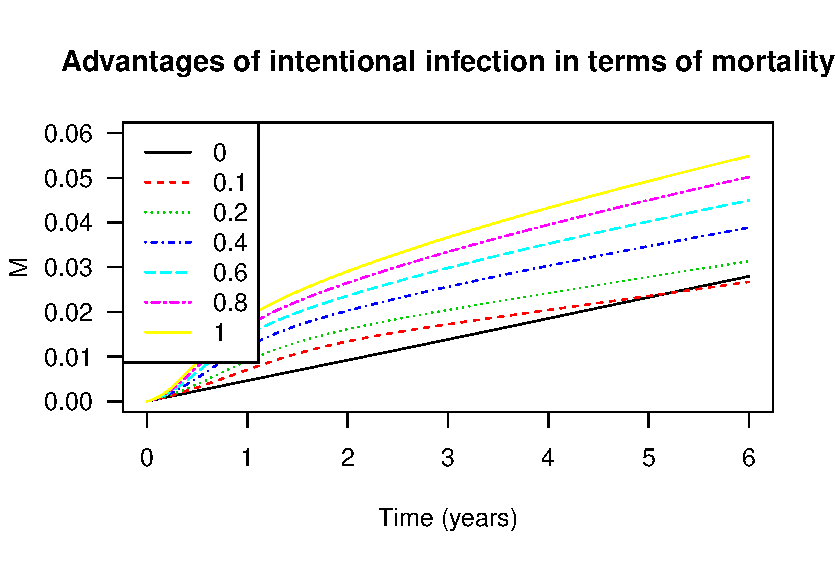
\includegraphics[width=0.9\textwidth]{Figures/dMdt.pdf}
%  \caption{An illustration of intentional infection have advantages over non-intentional infection}
%\end{figure}
%\end{frame}
%%%%%%%%%%%%%%%%%%%%%%%%%%%%%%%%%%%%%%%%%%%%%%%%%%%%
%%%%%%%%%%%%%%%%%%%%%%%%%%%%%%%%%%%%%%%%%%%%%%%%%%%%5
\begin{frame}
\begin{figure}[H]
  \centering
  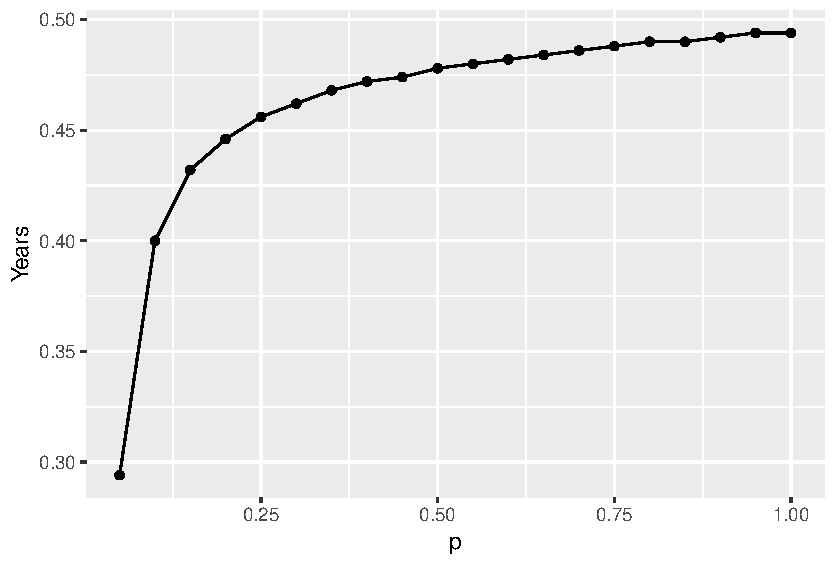
\includegraphics[width=0.7\textwidth]{Figures/Time_to_advantage_plot.pdf}
  \caption{Time to advantage, as a function of $p$}
\end{figure}
With a lower proportion of intentional infection, we can gain advantages relative faster.
\end{frame}
%%%%%%%%%%%%%%%%%%%%%%%%%%%%%%%%%%%%%%%%%%%%%%%%%%%%%
\begin{frame}
\frametitle{Possibility of disease eradication}

$\hat{I}=0$ at EE. We can consider the Naturally infected cases already been eradicated at EE.

\pause
For intentionally infected cases, if we stop intentional infection after we reach EE, can they burn out?
\end{frame}
%%%%%%%%%%%%%%%%%%%%%%%%%%%%%%%%%%%%%%%%%%%%%%%%%%%%%%
\begin{frame}
\frametitle{Possibility of disease eradication}

Vaccination threshold (Herd immunity): $p_c=1-\frac{1}{\R_0}$

\pause

\begin{center}
Threshold for susceptible: $S=\frac{1}{\R_0}$
\end{center}

\pause
If $S$ remains below this threshold until $V$ goes extinct, then we can achieve complete eradication of this disease.
\end{frame}
%%%%%%%%%%%%%%%%%%%%%%%%%%%%%%%%%%%%%%%%%%%%%%%%%%%%%
\begin{frame}
\frametitle{Possibility of disease eradication}

Example: $p=1$ initially, stop intentional infection after reaching EE, 
\begin{figure}[H]
  \centering
  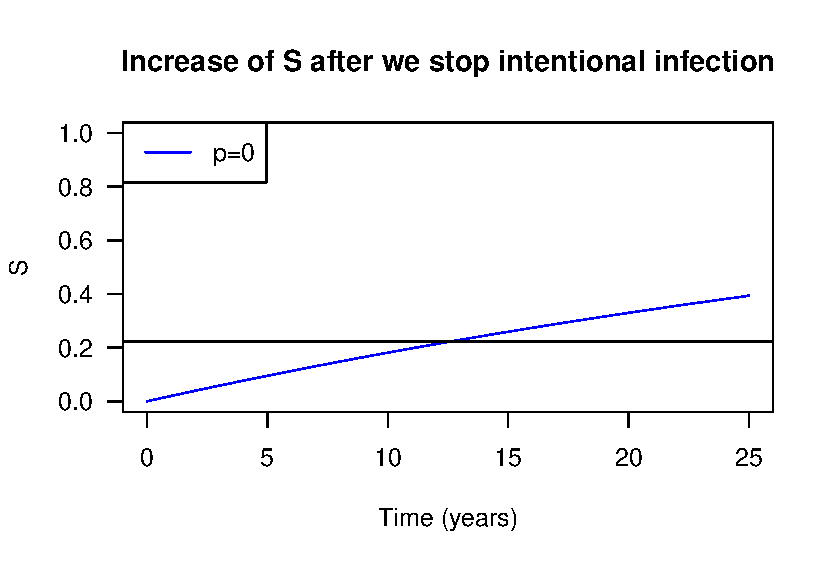
\includegraphics[width=0.75\textwidth]{Figures/Increase_of_S.pdf}
  \caption{For more than 10 years after we stop intentional infection, $S<\frac{1}{\R_0}$}
\label{figure:S_after_stop}
\end{figure}
\end{frame}
%%%%%%%%%%%%%%%%%%%%%%%%%%%%%%%%%%%%%%%%%%%%%%%%%%%%
\begin{frame}
\frametitle{Possibility of disease eradication}
\begin{figure}[H]
  \centering
  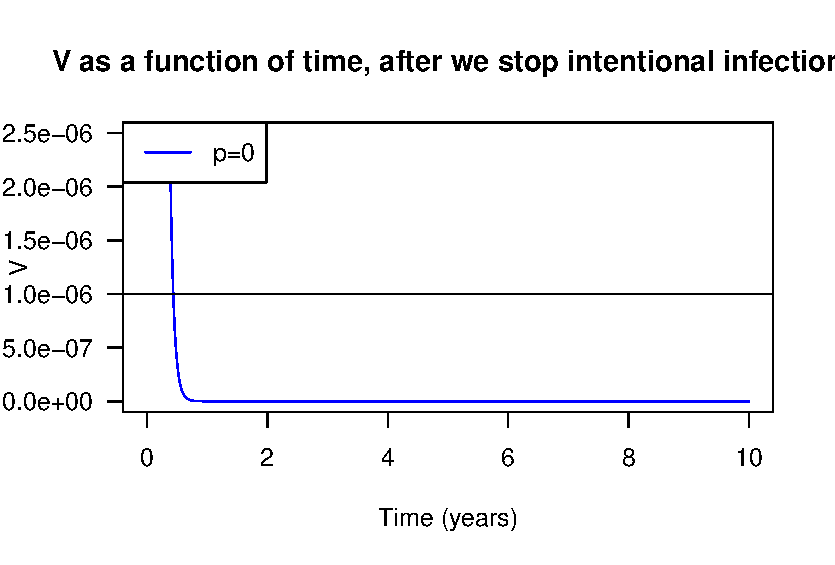
\includegraphics[width=0.8\textwidth]{Figures/V_after_stop.pdf}
  \caption{It takes less than 1 year for $V$ to fall below $1\times10^{-6}$}
\end{figure}
\end{frame}
%%%%%%%%%%%%%%%%%%%%%%%%%%%%%%%%%%%%%%%%%%%%%%%%%%%%%
\begin{frame}
\frametitle{Future expectation}
\begin{itemize}\itemsep10pt
\item Model extension
\pause
\begin{itemize}\itemsep10pt
\item Different transmission rate for intentionally or naturally infected cases
\pause
\item Different recovery rate
\end{itemize}
\pause
\item Combination of strategies
\pause
\item Comparison to traditional vaccination
\pause
\item Other strategies for intentional infection
\end{itemize}
\end{frame}
%%%%%%%%%%%%%%%%%%%%%%%%%%%%%%%%%%%%%%%%%%%%%%%%%%%%%
\begin{frame}
\frametitle{Other strategies for intentional infection}

Another approach would be to intentionally infect susceptible individuals, with a certain rate $r$.
\pause
\begin{equation}
\begin{split}
\dbyd{S}{t}&=\mu- \beta SI-rS-\mu S\,, \\
\dbyd{I}{t}&=rS+\beta SI-\gamma I -\mu I\,,\\
\dbyd{R}{t}&=\gamma I-\mu R\,,
\end{split}
\end{equation}
\end{frame}
%%%%%%%%%%%%%%%%%%%%%%%%%%%%%%%%%%%%%%%%%%%%%%%%%%%%%
\begin{frame}
\frametitle{Challenges to this method}
\begin{itemize}
\item Identify susceptible individuals
\end{itemize}
\end{frame}
%%%%%%%%%%%%%%%%%%%%%%%%%%%%%%%%%%%%%%%%%%%%%%%%%
\begin{frame}
\frametitle{Conclusion}
\begin{itemize}\itemsep10pt
\item Intentional infection has positive effects on population level disease control.
\item Further study is required for determining intentional infection strategies to optimize this method.
\end{itemize}
\end{frame}
%%%%%%%%%%%%%%%%%%%%%%%%%%%%%%%%%%%%%%%%%%%%%%%%%%%%%%%
\begin{frame}{References}
\begin{thebibliography}{9}
\bibitem{article}
Paulinevan den Driessche \emph{Reproduction numbers of infectious disease models}, Infectious Disease Modelling, Volume 2, Issue 3, August 2017, Pages 288-303.

\bibitem{article}
R.M. Anderson, R.M. May
\emph{Infectious diseases of humans: Dynamics and control}, Oxford University Press, Oxford, UK (1991)
\end{thebibliography}
\end{frame}
\end{document}

